\documentclass[a4paper,11pt]{article}

\usepackage{fancyhdr}
\usepackage[dvips]{graphicx}  % for eps and MatLab Diagrams
\usepackage{amsmath}
\usepackage{psfrag,color}
\usepackage[framed]{/Applications/TeX/mcode}
\usepackage{hyperref}

\pagestyle{fancy}

\begin{document} % Begin Document

% Title
\title{\textsc{Efficient Computation of the Fresnel Sine and Cosine Integrals}}

% Authors and Contact Information
\author{\textbf{John R. D'Errico}\\
Email: woodchips@rochester.rr.com}

\maketitle

\section{Abstract}
The goal of this exercise Is to find an efficient (fully vectorized) scheme for approximation of the Fresnel Sine and Cosine integrals, that is accurate to within 14 to 15 significant digits over the entire domain of interest.

\section{Introduction}

This document will describe an approach used to approximate the Fresnel sine and cosine integrals to as high a precision possible, while still maintaining maximal efficiency. To learn about the Fresnel integrals themselves, Wikipedia is often a reasonable place to start. (\url{http://en.wikipedia.org/wiki/Fresnel_integral})

There are three common forms for the integrals themselves, all essentially simple transformations of the others. Thus the cosine integral is usually written in one of these forms...

\begin{equation}
    C(x) = \int_0^x cos(\frac{\pi t^2}{2}) dt
\end{equation}

\begin{equation}
    C_1(x) = \sqrt(\frac{2}{\pi}) \int_0^x cos(t^2) dt
\end{equation}

\begin{equation}
    C_2(x) = \frac{1}{\sqrt{2 \pi}} \int_0^x \frac{cos(t)} {\sqrt{t}} dt
\end{equation}

\begin{figure}
\centering
    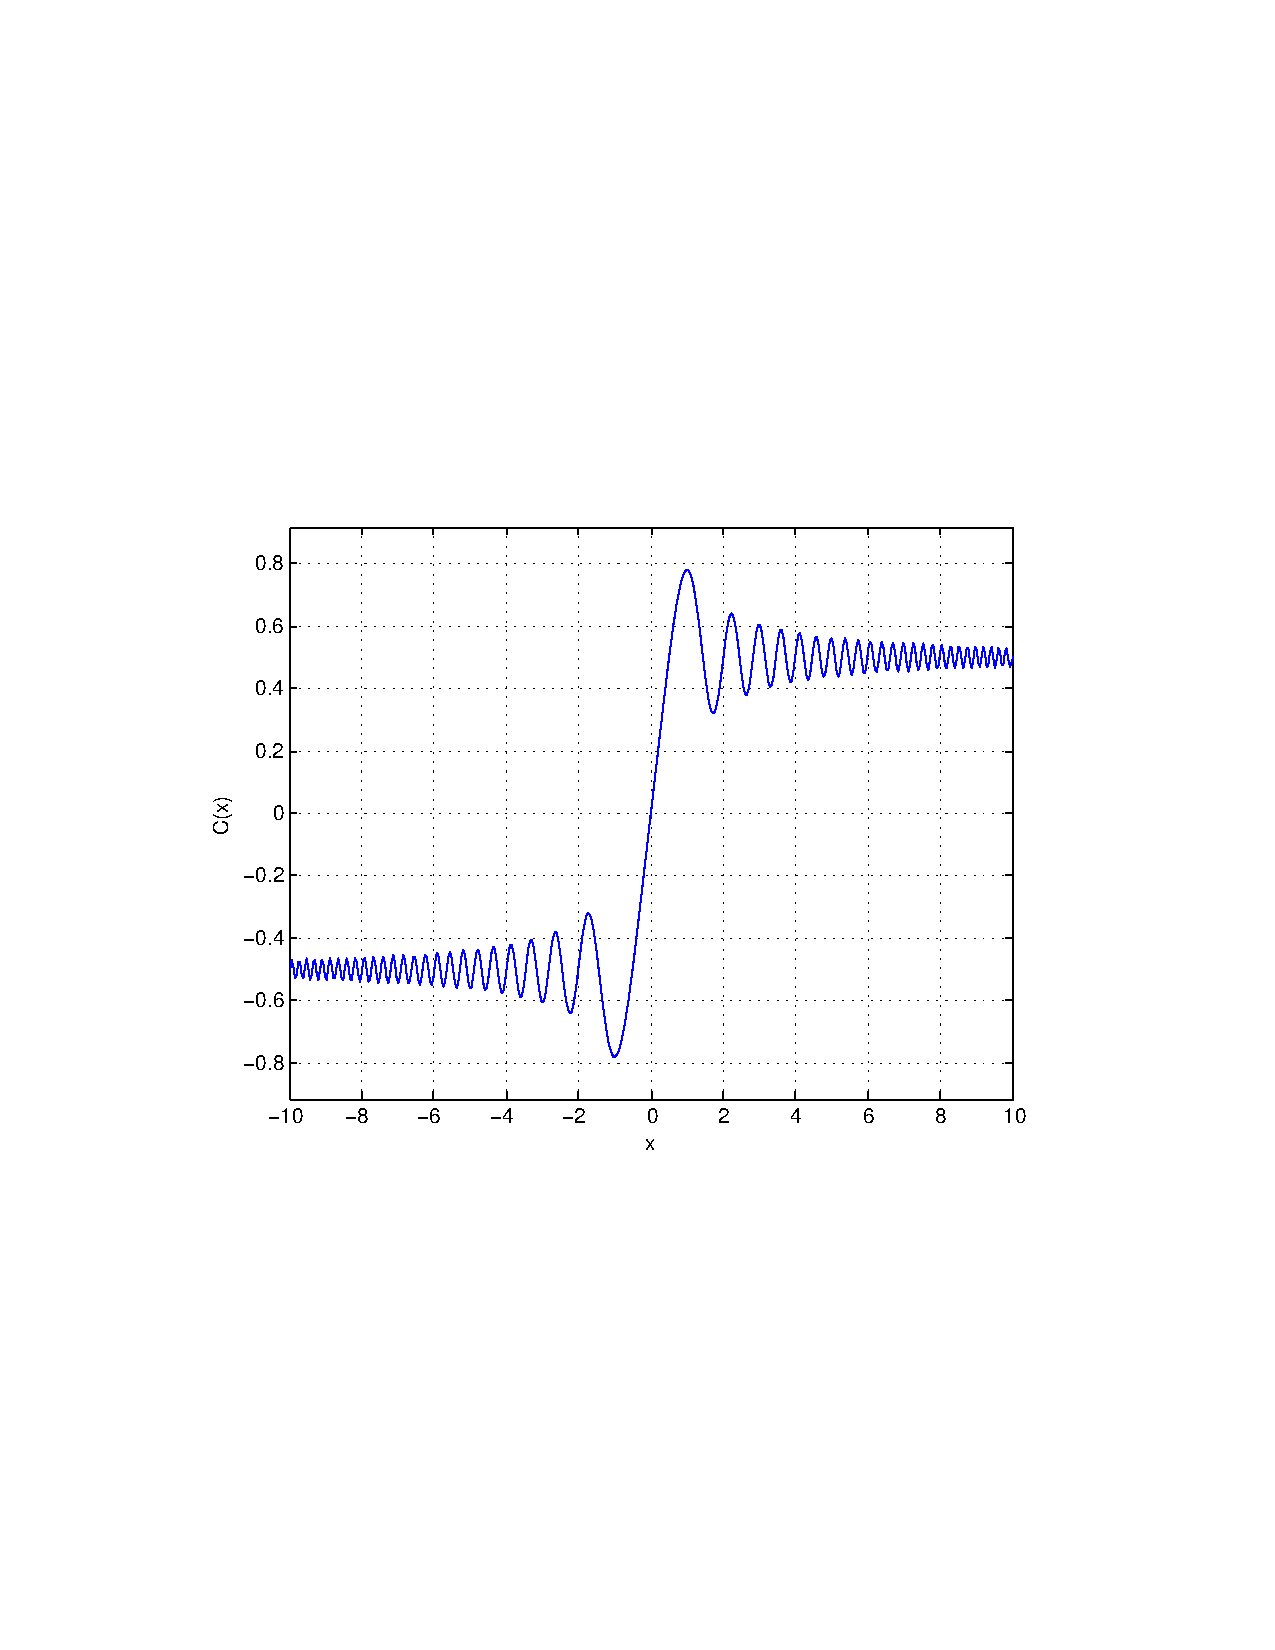
\includegraphics[width=5in]{C.pdf}
        \caption{Fresnel cosine integral, C(x)}
\end{figure}

And, the sine integral appears in one of these forms...

\begin{equation}
    S(x) = \int_0^x sin(\frac{\pi t^2}{2}) dt
\end{equation}

\begin{equation}
    S_1(x) = \sqrt(\frac{2}{\pi}) \int_0^x sin(t^2) dt
\end{equation}

\begin{equation}
    S_2(x) = \frac{1}{\sqrt{2 \pi}} \int_0^x \frac{sin(t)} {\sqrt{t}} dt
\end{equation}

\begin{figure}
\centering
    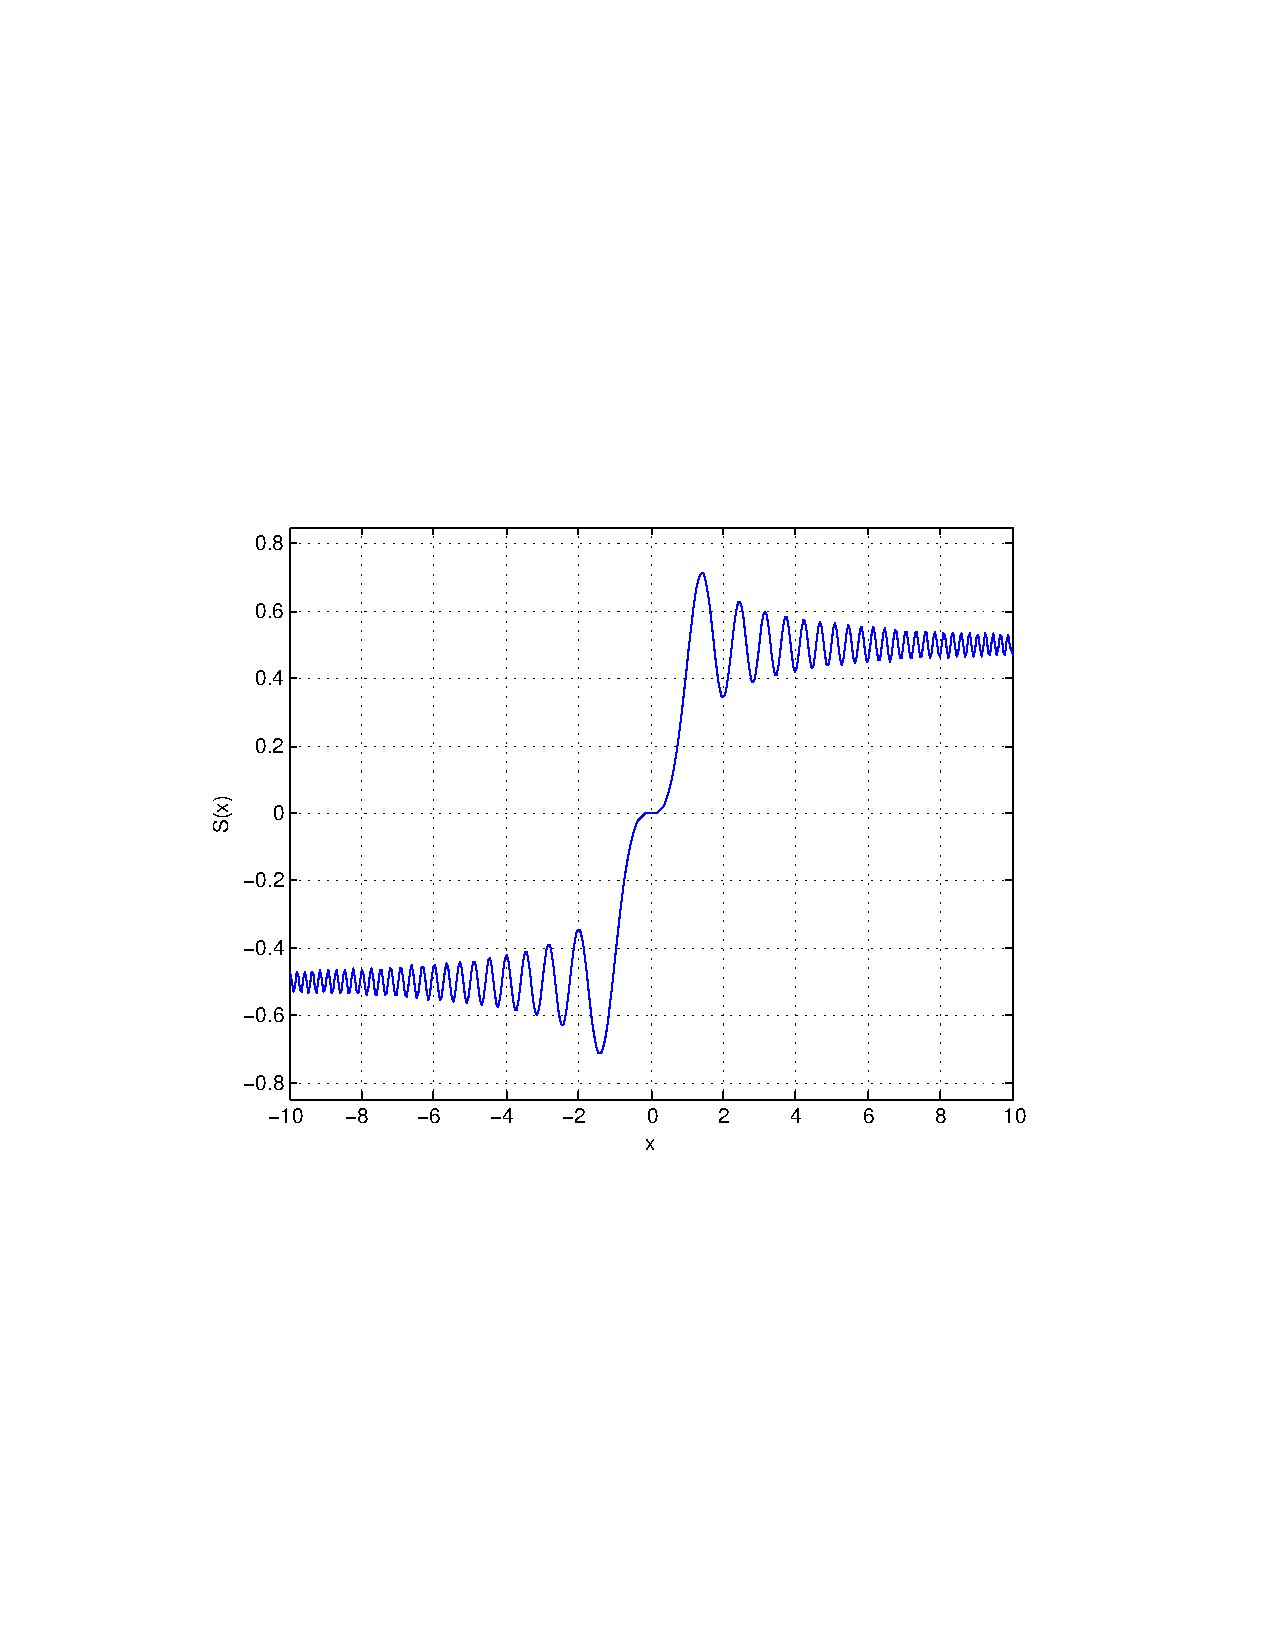
\includegraphics[width=5in]{S.pdf}
        \caption{Fresnel sine integral, S(x)}
\end{figure}

As one might expect, these integrals are oscillatory beasts, converging eventually to a limit for both $C(X)$ and $S(X)$ of $1/2$ as x grows large.

Some simple approximations are found in Abramowitz and Stegun [1], as well as a set of tables one might use to interpolate these integrals. The goal of this investigation is to develop an efficient, (fully vectorized) scheme for evaluating the integrals as a function of any real value for the end point. Understanding the techniques used is of value for other problems.


\section{Numerical approximation: adaptive quadrature using quadgk}

Numerical computation of the Fresnel sine and cosine integrals poses an interesting problem. While there are accurate approximations to be found for small values of the arguments as well as large, it is for intermediate values that difficulties arise. But before I go too far, it is first important to be able to compute the actual value of these integrals for any end point. Luckily, in MATLAB the simple way to compute such an integral is via an adaptive numerical integration. The function quadgk is a good choice here.

\begin{lstlisting}
>> FresnelCObj = @(t) cos(pi*t.^2/2);
>> quadgk(FresnelCObj,0,1,'abstol',1e-15)
ans =
         0.779893400376823
\end{lstlisting}

In fact, quadgk is pretty efficient, and it provides us with an accurate way to get ground truth estimates for these integrals. Here I'll use timeit for a time estimate, a function written by Steve Eddins, provided on the MATLAB Central file exchange.

\begin{lstlisting}
>>timeit(@() quadgk(FresnelCObj,0,9,'abstol',1e-15))
ans =
             0.00094665522
\end{lstlisting}    

If I compare the time required to my own final code for a single value, I see that quadgk is really quite fast in terms of the time required. Since quadgk is doing an adaptive numerical integration of a highly oscillatory function, that time of 0.00095 seconds seems fast to me.

\begin{lstlisting}
>> timeit(@() fresnelC(9,0))
ans =
             0.00011972314
\end{lstlisting}

In fact, one might argue that quadgk is fast enough that there is no reason to provide a better solution. This argument fails on two points. First, adaptive quadrature fails for seriously large upper limits on the integral, because the oscillations get more rapid for those larger values. Even values as large as 100 will cause problems.

\begin{lstlisting}
>> quadgk(FresnelCObj,0,100,'abstol',1e-16)
Warning: Reached the limit on the maximum number of intervals in use.
Approximate bound on error is  1.3e+01. The integral may not exist, or
it may be difficult to approximate numerically. Increase MaxIntervalCount
to 970 to enable QUADGK to continue for another iteration. 
> In quadgk>vadapt at 317
  In quadgk at 208
ans =
         0.513404445484837
\end{lstlisting}

Second, a vectorized code should be more efficient than simply wrapping a loop around that code. So if one call to quadgk takes roughly 0.0009 seconds, then 1000 calls will take 0.9 seconds. However, at least careful application of quadgk will yield good ground truth estimates to test any approximations we choose.

\section{Numerical approximation: series approximations}

We can look in Abramowitz and Stegun [1] for series approximations to these Fresnel integrals. For example, for small values of x, series approximations work reasonably well. (7) is given as Abramowitz and Stegun (7.3.11). 

\begin{equation}
    C(x) = \sum_{n=0}^N \frac{(-1)^n (\pi/2)^{2n}}{(2n)! (4n+1)} x^{4n+1}
\end{equation}

While the series (7) is convergent for all x, how many terms are required? Figure 3 shows the approximate number of terms in that series required for the magnitudes of those individual terms in the alternating series to drop below $10^{-16}$. As such, this approximation will only be useful for small values of x.

\begin{figure}
\centering
    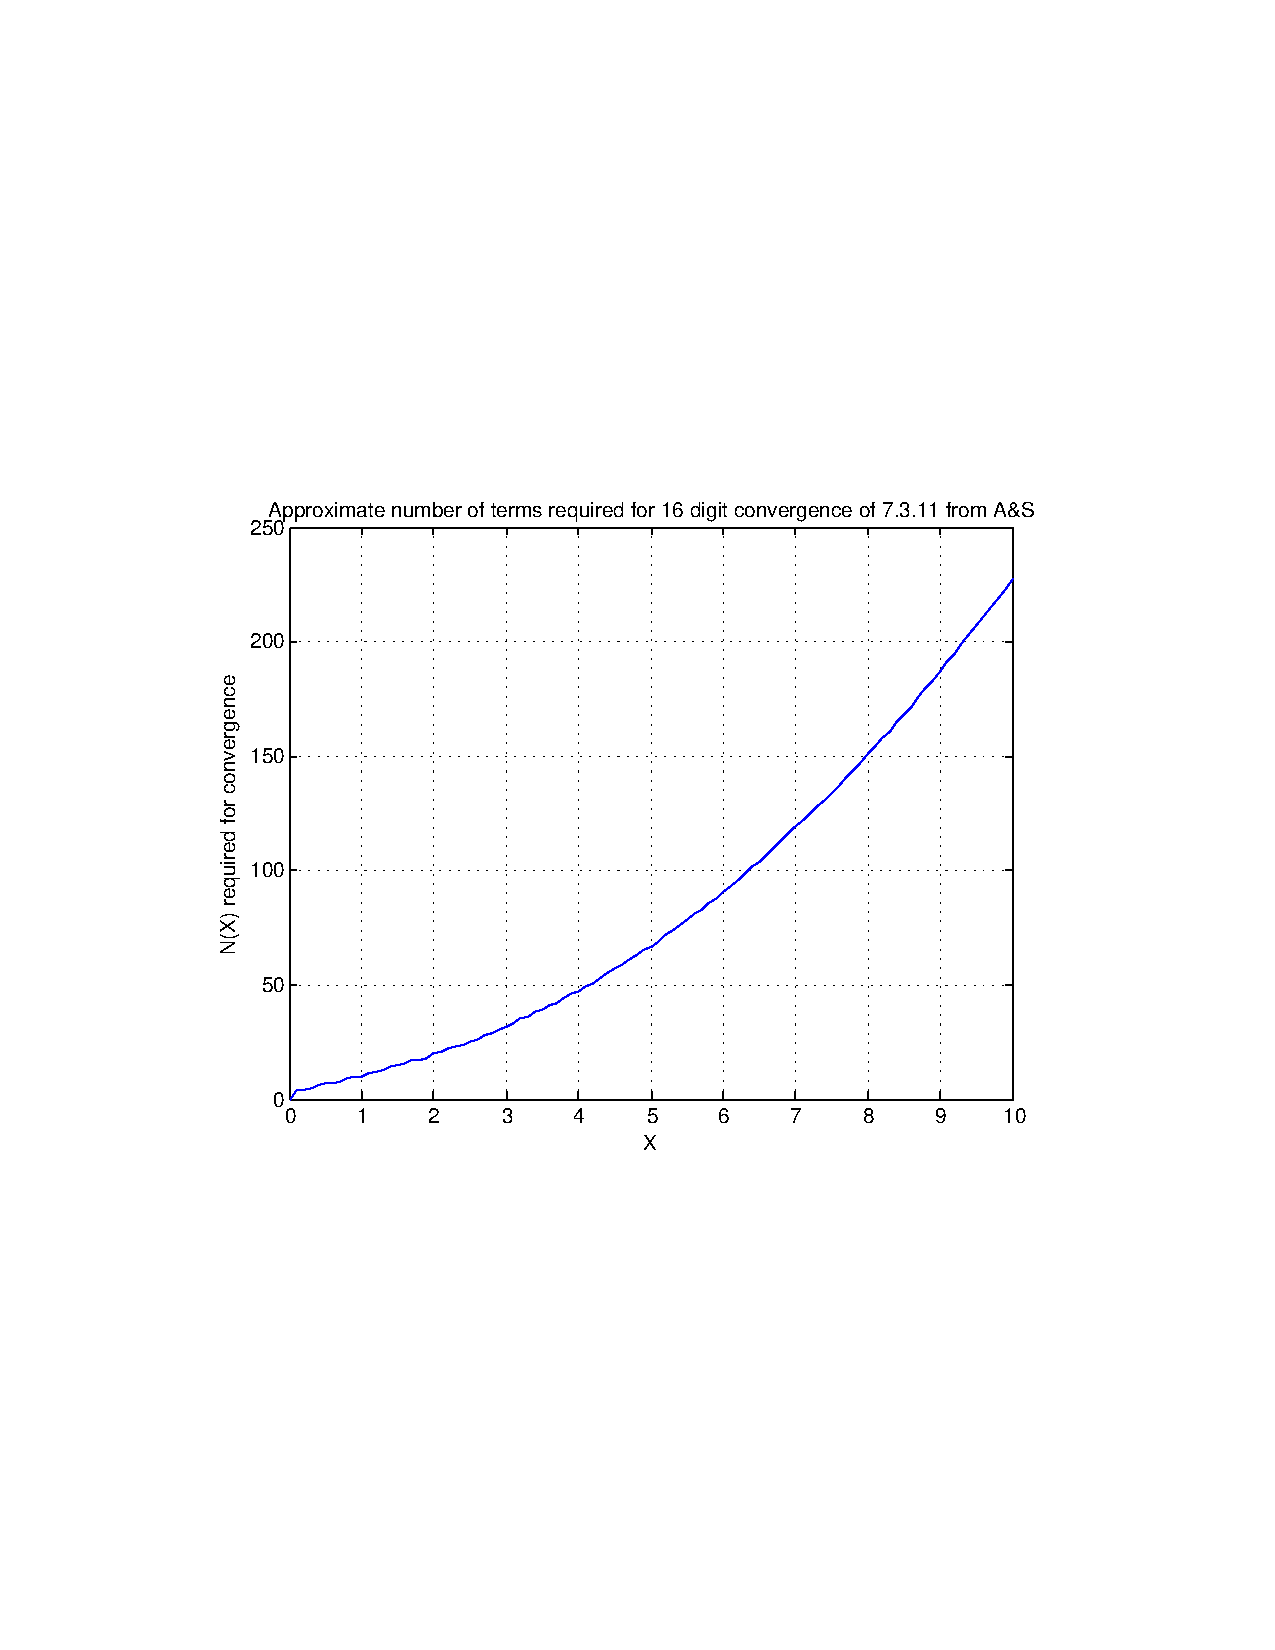
\includegraphics[width=5in]{Convergence7311.pdf}
        \caption{Terms required for convergence of Abramowiz and Stegun 7.3.11 for C(x)}
\end{figure}

There are also useful series approximations (Mielenz [2]) that are good for large values of x. A pair of auxilliary functions $f(x)$ and $g(x)$, associated with the sine and cosine integrals provide those approximations.

\begin{equation}
    C(x) = 1/2 + f(x) sin(\frac{\pi t^2}{2}) - g(x) cos(\frac{\pi t^2}{2})
\end{equation}

\begin{equation}
    S(x) = 1/2 - f(x) sin(\frac{\pi t^2}{2}) - g(x) cos(\frac{\pi t^2}{2})
\end{equation}

These auxilliary functions are useful because they are expressible in series using {\it negative} powers of x. These series are rapidly convergent for even moderately large values of x. In fact, they offer essentially full double precision accuracy for x as small as 7.5 after only 5 terms.

\begin{equation}
f(x) = \sum_{n=0} \frac{(-1)^n (4n)! } {(2n)! 2^{2n}  \pi^{2n+1} x^{4n+1}}
\end{equation}

\begin{equation}
g(x) = \sum_{n=0} \frac{(-1)^n (4n+2)! } {(2n+1)!  2^{2n+1}  \pi^{2n+2} x^{4n+3}}
\end{equation}

Expanded to a few terms, we get (12) and (13).

\begin{equation}
f(x) = \frac{1}{\pi x} - \frac{3}{\pi^3 x^5} + \frac{105}{\pi^5 x^9}  - \frac{10395}{\pi^7 x^{13}} + \frac{2027025}{\pi^9 x^{17}} + \epsilon(x)
\end{equation}

\begin{equation}
g(x) =  \frac{1}{\pi^2 x^3} - \frac{15}{\pi^4 x^7} + \frac{945}{\pi^6 x^{11}}  - \frac{135135}{\pi^8 x^{15}} + \frac{34459425}{\pi^{10} x^{19}} + \delta(x)
\end{equation}

Because $f(x)$ and $g(x)$ from (12) and (13) seem so well behaved for relatively large x, for what range of values of x can we use these approximations?

\begin{figure}
\centering
    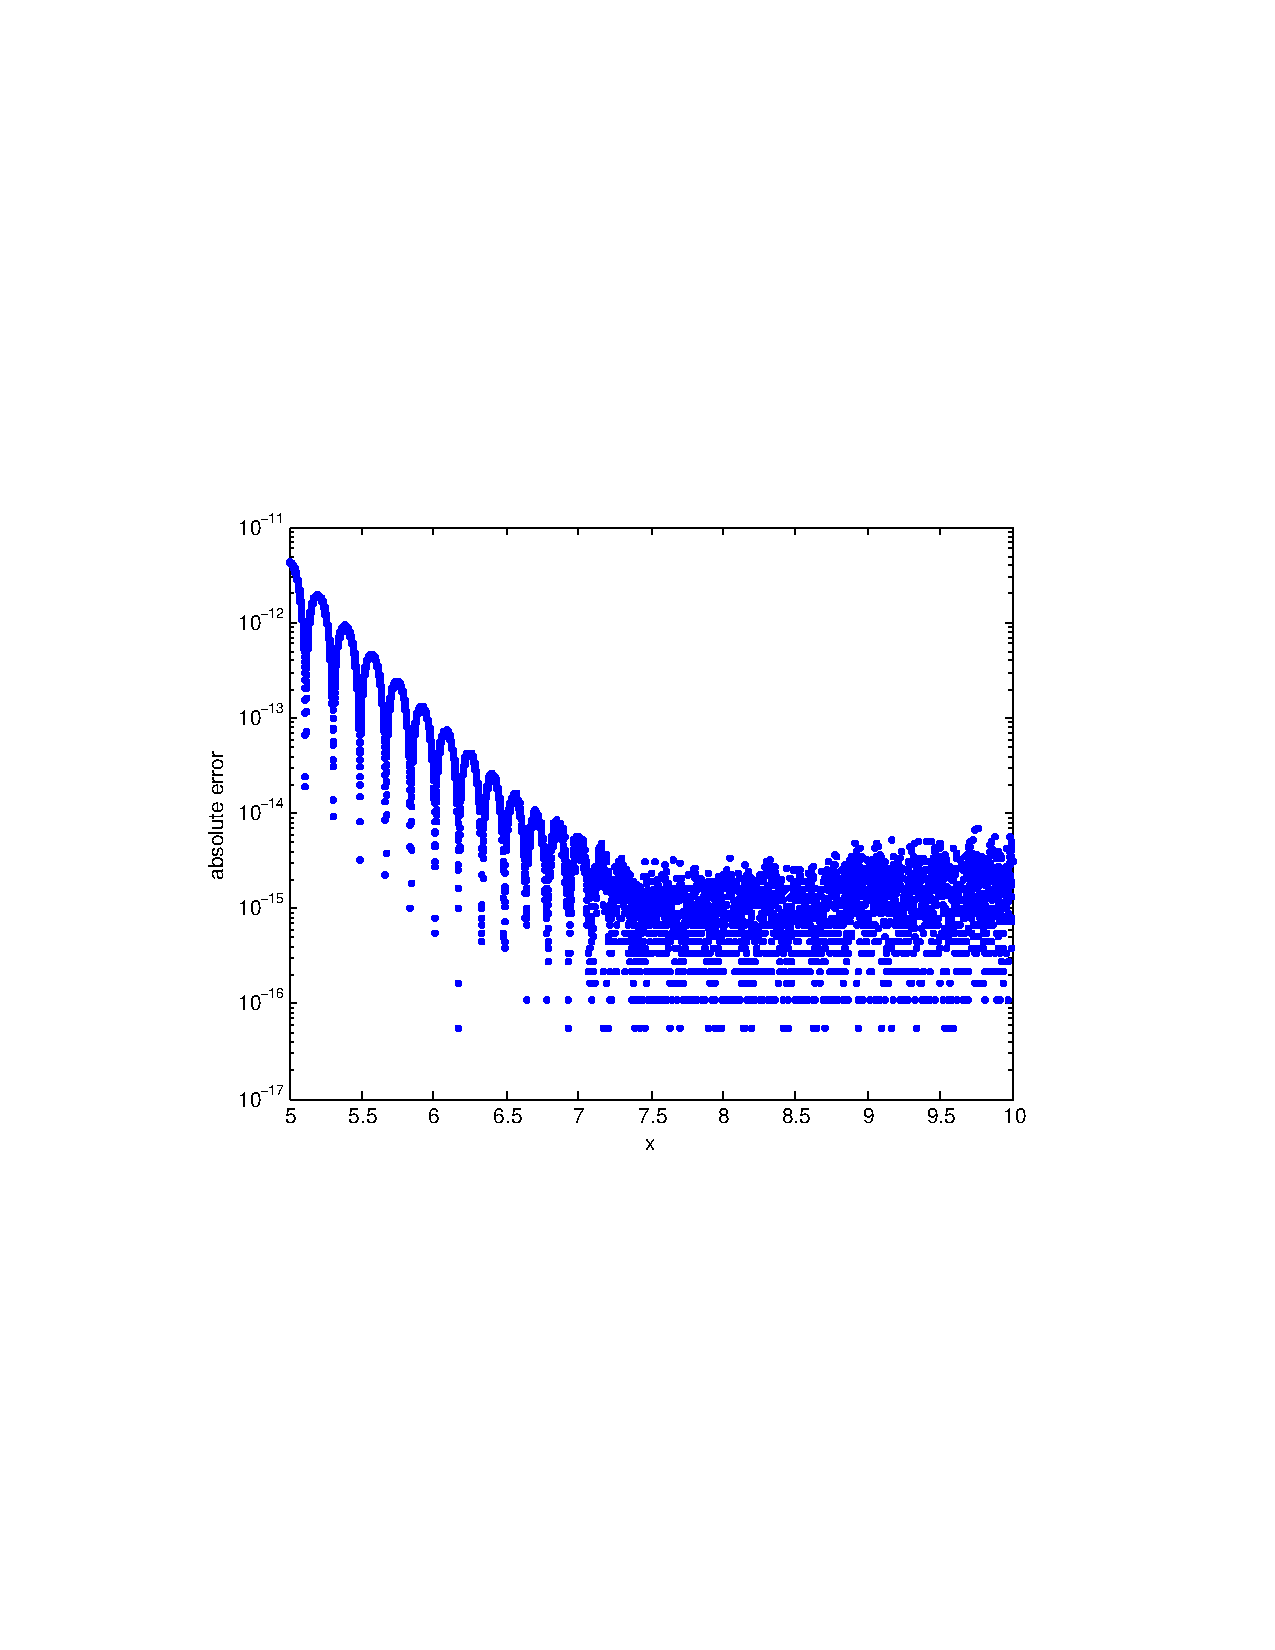
\includegraphics[width=5in]{associatedfgerrors.pdf}
        \caption{Absolute error for (12) when used to approximate C(x)}
\end{figure}

In Figure 4, we see the absolute error in C(X), when (12) and (13) are used, combined with (8) to approximate $C(x)$. Plotted on a log scale in y, we see that the predicted error is dominated by a sinusoidal component for x below roughly 7. For x above that point, it degenerates into noise. This seems to be clearly the error in the ability of our adaptive numerical integration to compute ground truth. As well, once the error approaches the vicinity of $10^{-16}$, we begin to approach the fundamental limits of what a double precision computation can supply.

This suggests that while (8), (9), (12), (13) can be combined to yield excellent approximations for moderately large values of x (i.e., $x > 7.5$), we still need a viable method for smaller values of x. While Mielenz chooses better approximations for f and g for even smaller values of x, the approach they used will likely not easily yield the double precision accuracy that is the aim of this study.


\section{Numerical approximation: spline approximations}

The problem we saw in the previous chapter is that while series approximations exist for both moderately large and small values of x, there are none that adequately cover the ground between. To solve that problem, one could simply choose a spline interpolant of some sort. For example, Abramowitz and Stegun provides a simple set of tables for both the Fresnel sine and cosine integrals, tabulated for values of x over the interval [0,5], with a spacing of 0.02. One issue with a high accuracy approximation is these tables are only accurate to roughly seven significant digits. So any interpolant can be no higher accuracy than that if we start from those tables. Of course, the tables themselves can be recreated to a higher precision using a tool like quadgk. But how well can we do with a spline? And what kind of spline might we choose to gain the highest accuracy?

The tables provided by Abramowitz and Stegun were generated at a step of 0.02. So the first thing to do is to recompute those tables to have maximal double precision accuracy. quadgk will do this well enough for us.

\begin{lstlisting}
FresnelCKernel = @(t) cos(pi*t.^2/2);
x0 = 0:.02:7.5;
FC0 = zeros(size(x0));
for i = 1:numel(x0)
  FC0(i) = quadgk(FresnelCKernel,0,x0(i), ...
       'abstol',1e-16,'reltol',100*eps('double'));
end
\end{lstlisting}

Next, use a simple interpolant to provide intermediate values at any point. The MATLAB function interp1, when used with the 'cubic' method is equivalent to a pchip interpolant pchip on that set of points. Thus figure 5 shows the log of the absolute errors for a pchip interpolant over the interval [0,7.5].

\begin{figure}
\centering
    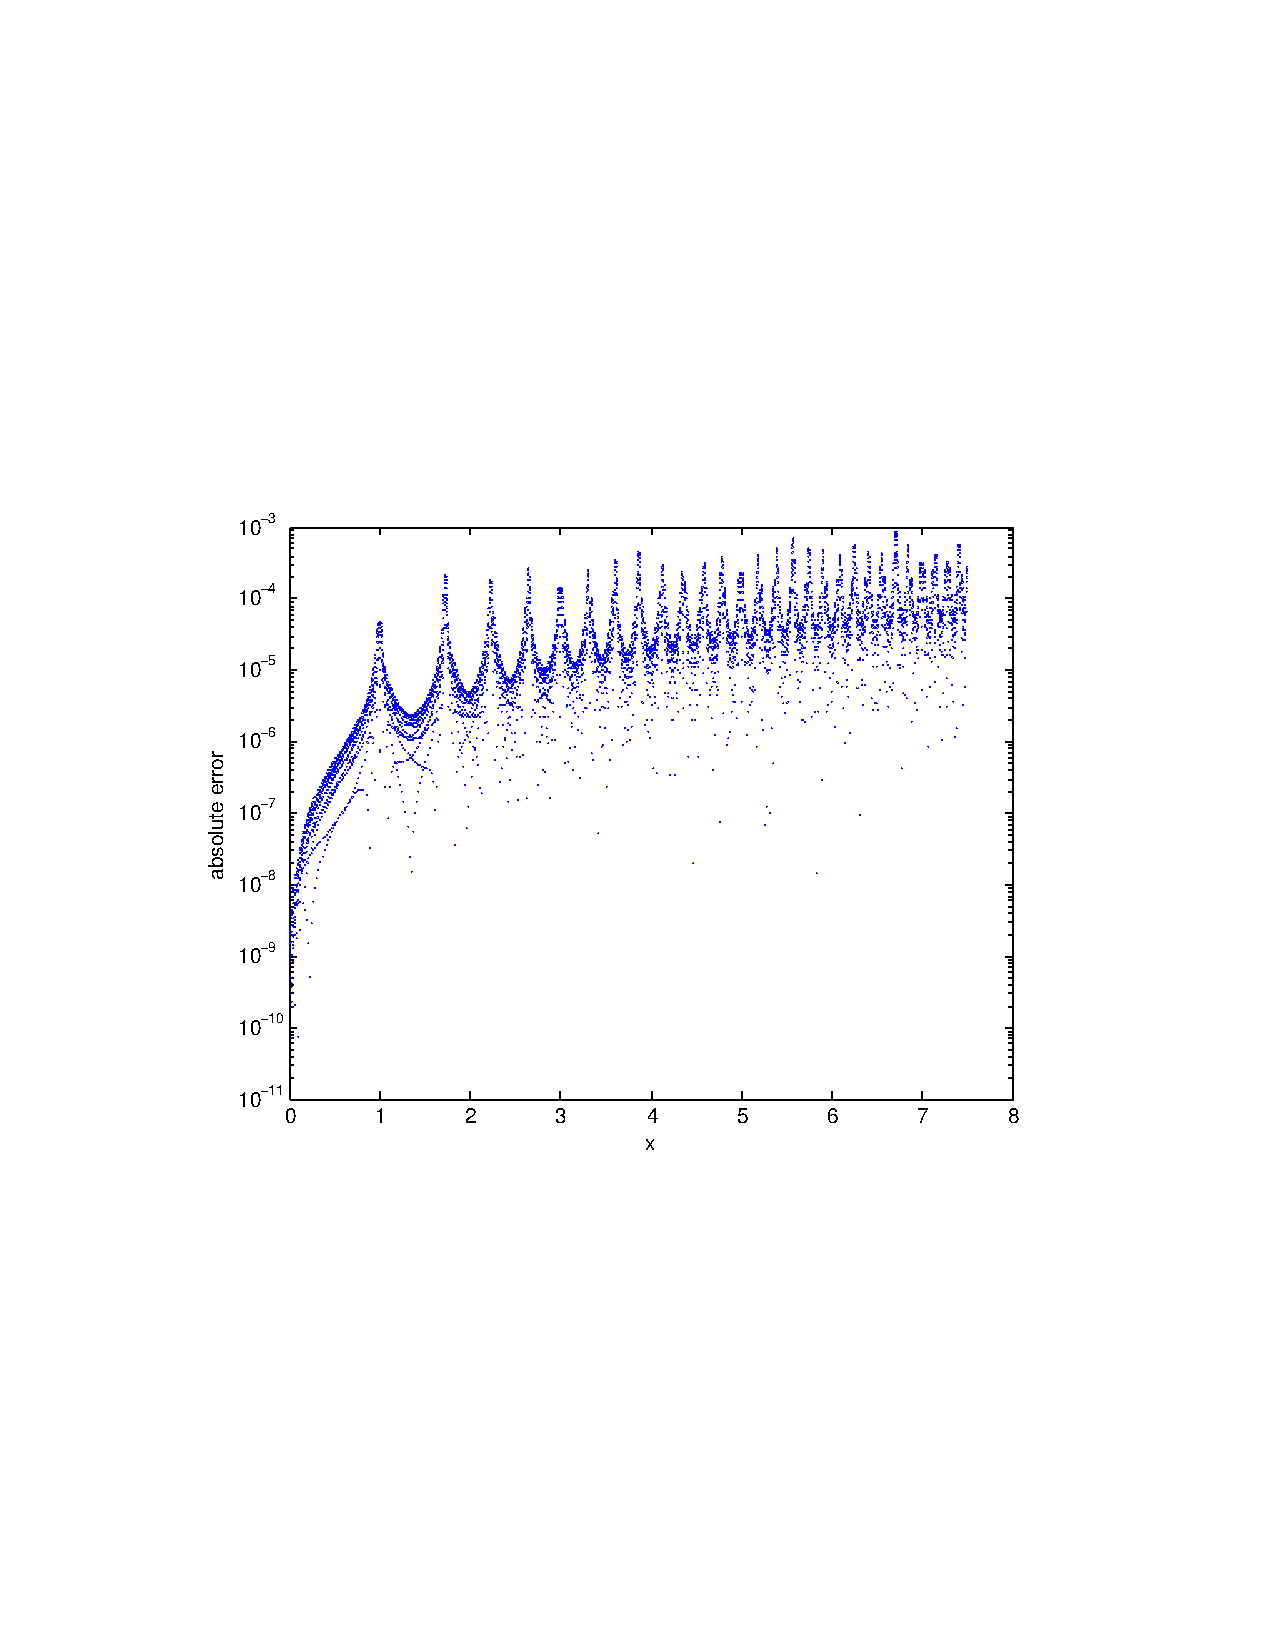
\includegraphics[width=5in]{pchiperrors.pdf}
        \caption{Absolute error for a pchip interpolant used to approximate C(x), step size was fixed at 0.02}
\end{figure}

There are two important things to learn from figure 5. First, that the error for a pchip interpolant with knot spacing of 0.02 will not give us the nearly 15 digits of accuracy that we look for. Secondly, because the function is an osculatory one that oscillates more rapidly at large values of x, the knots of the spline must themselves be placed at a tighter spacing as x grows larger. First, we can try using a cubic spline. The SPLINE function provided in MATLAB is a twice continuously differentiable cubic spline, as opposed to the $C_1$ function we get from PCHIP.

\begin{figure}
\centering
    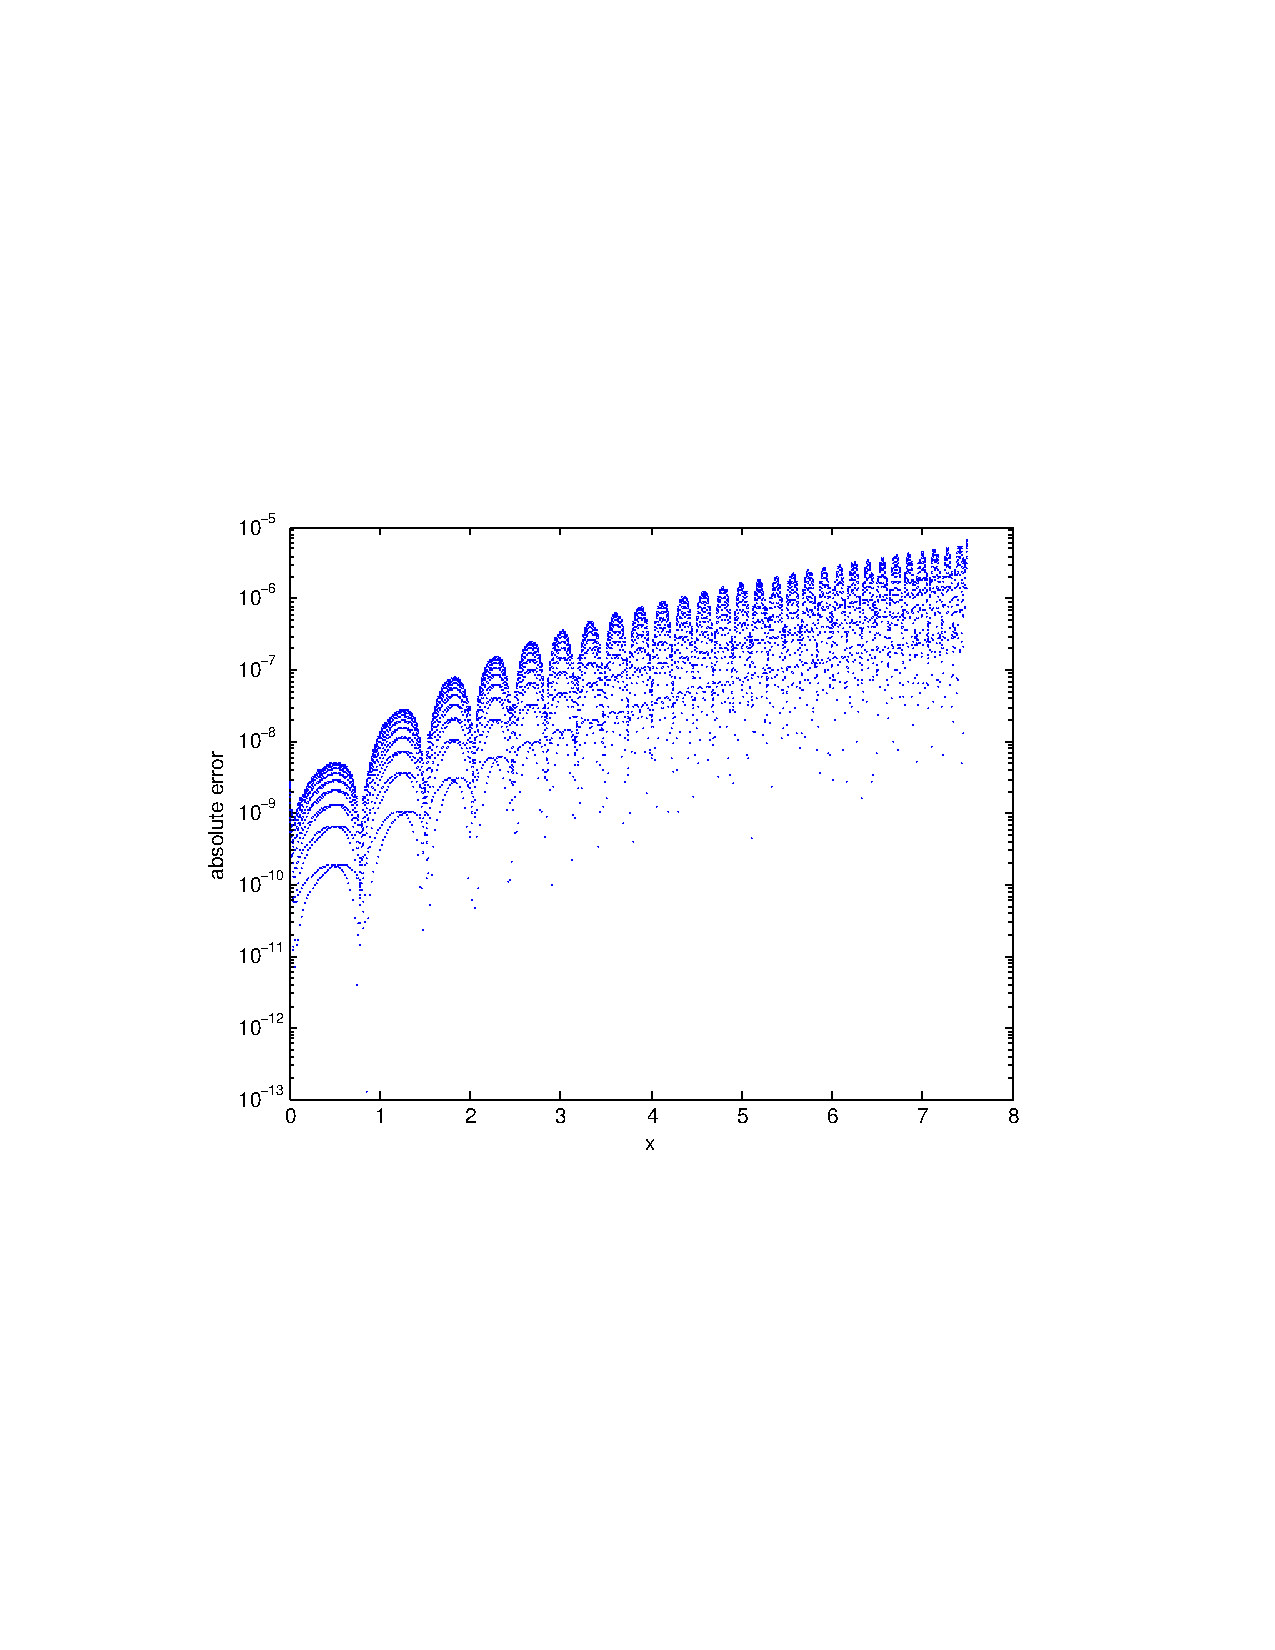
\includegraphics[width=5in]{cubicsplineerrors.pdf}
        \caption{Absolute error for a cubic spline interpolant used to approximate C(x), step size was fixed at 0.02}
\end{figure}

While we get several more digits of accuracy from this interpolant, it is insufficient. The next improvement is to use a nonlinear spacing for the tabulated data. For a similar table size, the best spacing for that table will yield no better errors than a bit less than $10^{-6}$ as a maximum.

\begin{lstlisting}
FresnelCKernel = @(t) cos(pi*t.^2/2);
p = 1.75;
n0 = 360;
x0 = linspace(1,7.5^p,n0).^(1/p);
dx = x0(2) - x0(1);
x0 = [linspace(0,1,ceil(1./dx)),x0];
FC0 = zeros(size(x0));
for i = 1:numel(x0)
  FC0(i) = quadgk(FresnelCKernel,0,x0(i), ...
       'abstol',1e-16,'reltol',100*eps('double'));
end
\end{lstlisting}

\begin{figure}
\centering
    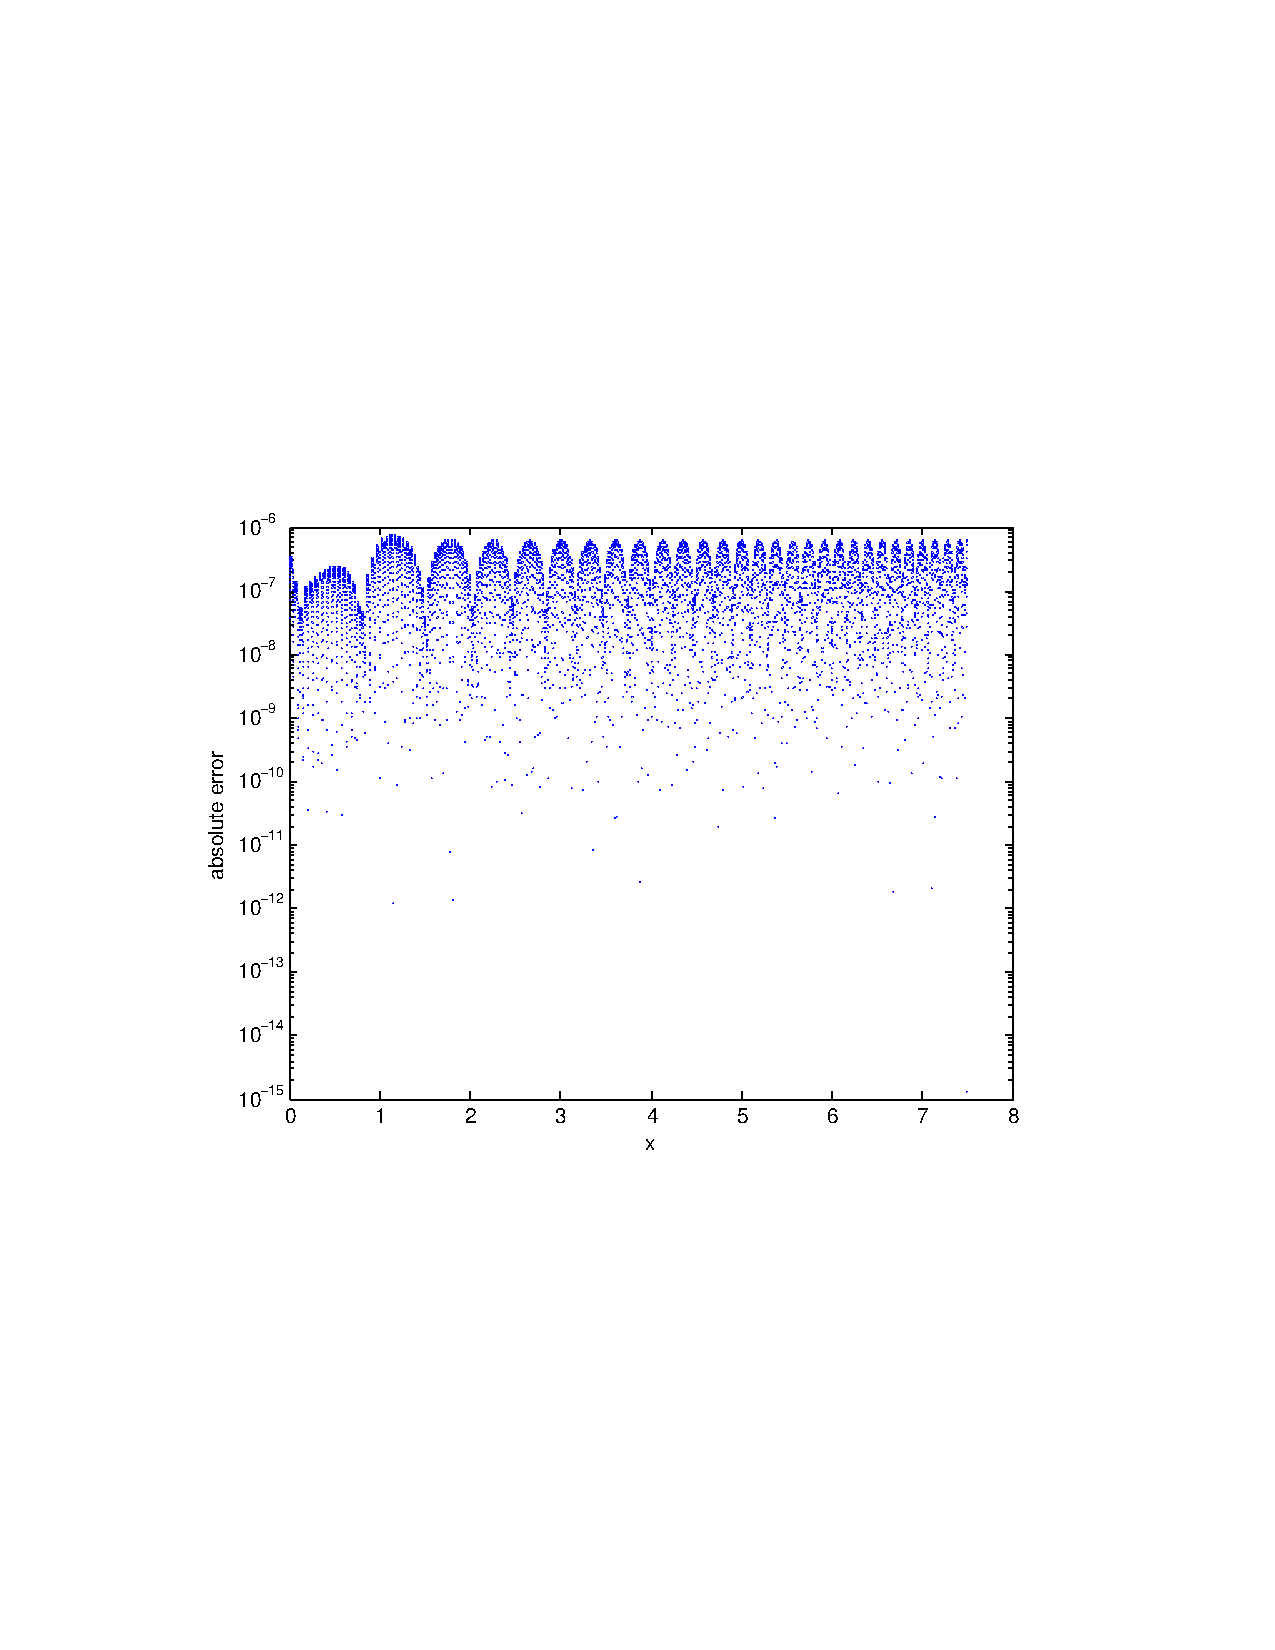
\includegraphics[width=5in]{unequallyspacedspline.pdf}
        \caption{Absolute error for a cubic spline interpolant used to approximate C(x) from an unequally spaced table}
\end{figure}

Another trick is to use a Hermite interpolant as opposed to an a spline itself. A spline uses only information about function values at the break points to infer the shape of the curve by presuming the function must be smooth. Can we do better if we supply the first derivatives of the function? Of course, here the first derivative of the sine and cosine integrals is just the value of the integrand evaluated at the upper limit of integration. As it turns out, this gains little improvement over a simple cubic spline, but we can easily enough extend this idea to a quintic Hermite function. Figure 8 shows the interpolation error for a quintic Hermite interpolant using a nonlinearly spaced interpolation table.

\begin{figure}
\centering
    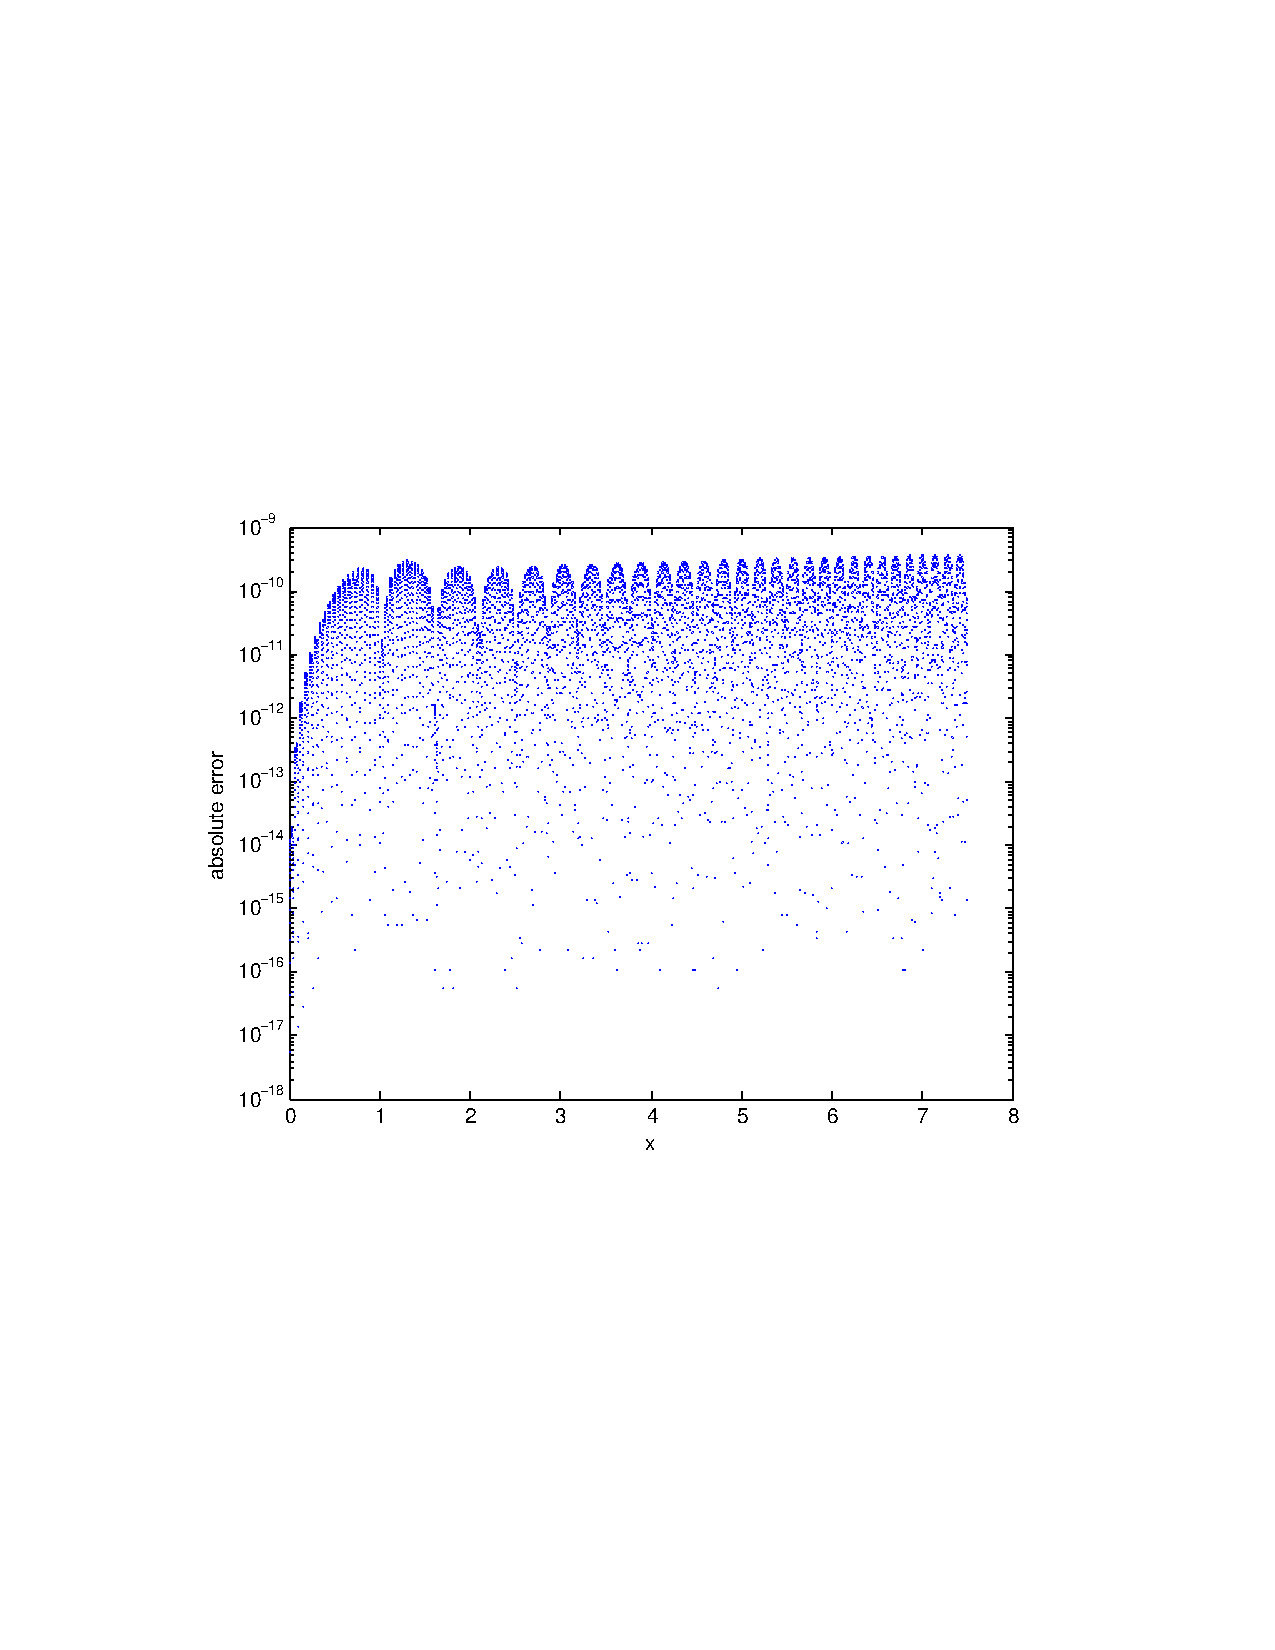
\includegraphics[width=5in]{quinticHermite.pdf}
        \caption{Absolute error for a piecewise quintic Hermite interpolant used to approximate C(x) from the unequally spaced table}
\end{figure}

Only a bit more work lets us gain an interpolation error that is generally no larger than $10^{-14}$, extending the order to a 7th degree Hermite interpolant, achieved by specifying the second and third derivatives at a slightly finer spacing for the final table. The result is a piecewise heptic interpolant with 527 break points, yielding an interpolation accuracy that is roughly as good as that achieved by the series approximation shown in figure 4 for x greater than 7.5.

\begin{figure}
\centering
    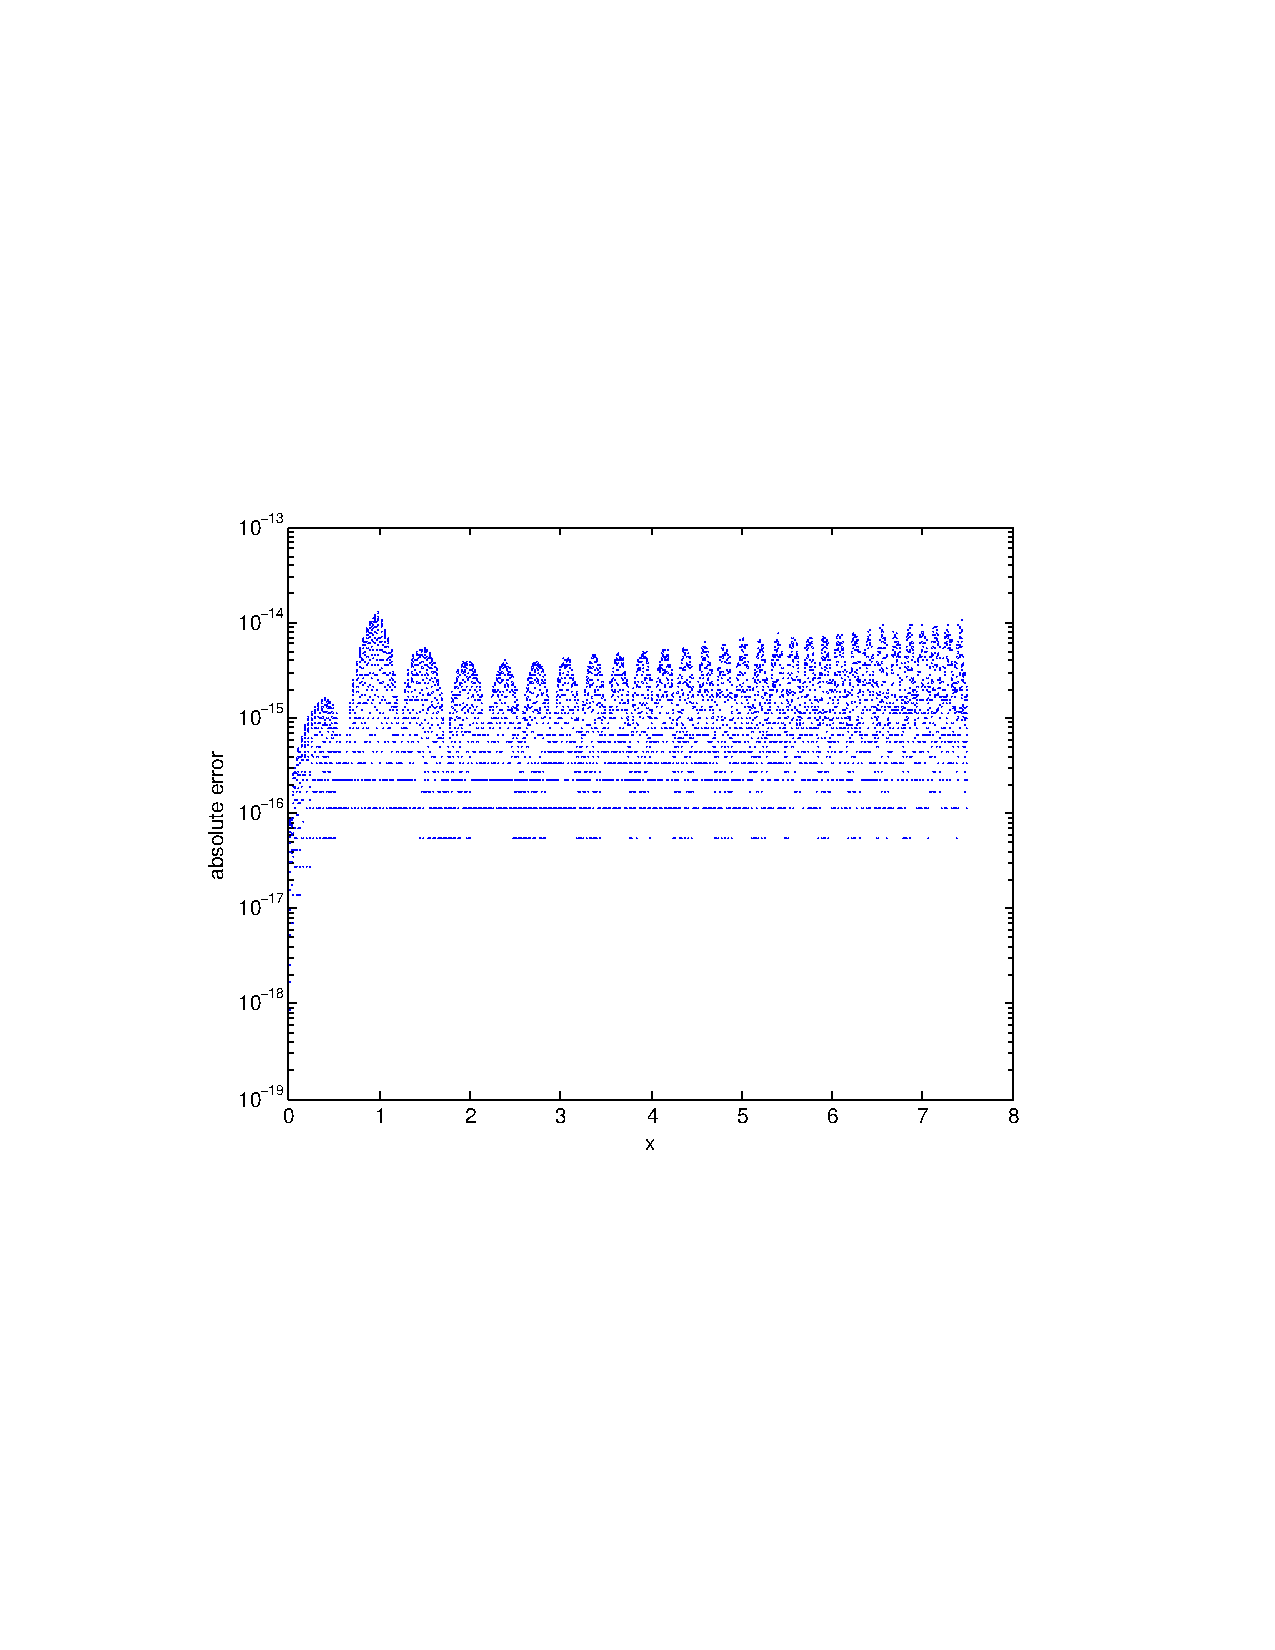
\includegraphics[width=5in]{hepticHermite.pdf}
        \caption{Absolute error for a piecewise 7th degree (heptic?) Hermite interpolant used to approximate C(x) from the unequally spaced table}
\end{figure}


\section{MATLAB Implementation}
The trick to implementing the approximations discussed in this note is simple. For any value of x at least as large as 7.5, use the associated function approximations given in (12) and (13), then (8( and (9) will yield an accuracy of roughly 14 significant digits. For smaller values of x, the 7th degree spline model is generated and stored in a .mat file, rather than recreating the splines on the fly. Those splines can be read in once in a matlab session, then stored in persistent variables. This makes the operation of this function quite efficient, yielding as close as possible full double precision accuracy for all values of x.



\section{References}

[1] Abramowitz, M. and Stegun, I. A. (Eds.). "Error Function and Fresnel 
      Integrals." Ch. 7 in Handbook of Mathematical Functions with
      Formulas, Graphs, and Mathematical Tables, 9th printing. New York:
      Dover, pp. 295-329, 1970.
 
[2] Mielenz, K. D.; "Computation of Fresnel Integrals", Journal of
      Research of the National Institute of Standards and Technology,
      Vol 102, Number 3, May-June 1997
         http://nvl.nist.gov/pub/nistpubs/jres/102/3/j23mie.pdf



\end{document}
